    \section{Development}
    This part contain all informations needed to develop new programs in BTK.

    \subsection{BTK tree}
    BTK is build using a tree.
    The source code is contained into the \textit{Code} folder.
    Programs are respectively into \textit{Applications} and \textit{Utilities}.
    \textit{Documentation} and \textit{Medias} contain the documentation and some pictures for the \href{http://rousseau.github.com/fbrain/}{Website of the project}

    \begin{figure}[H]
     \centering
      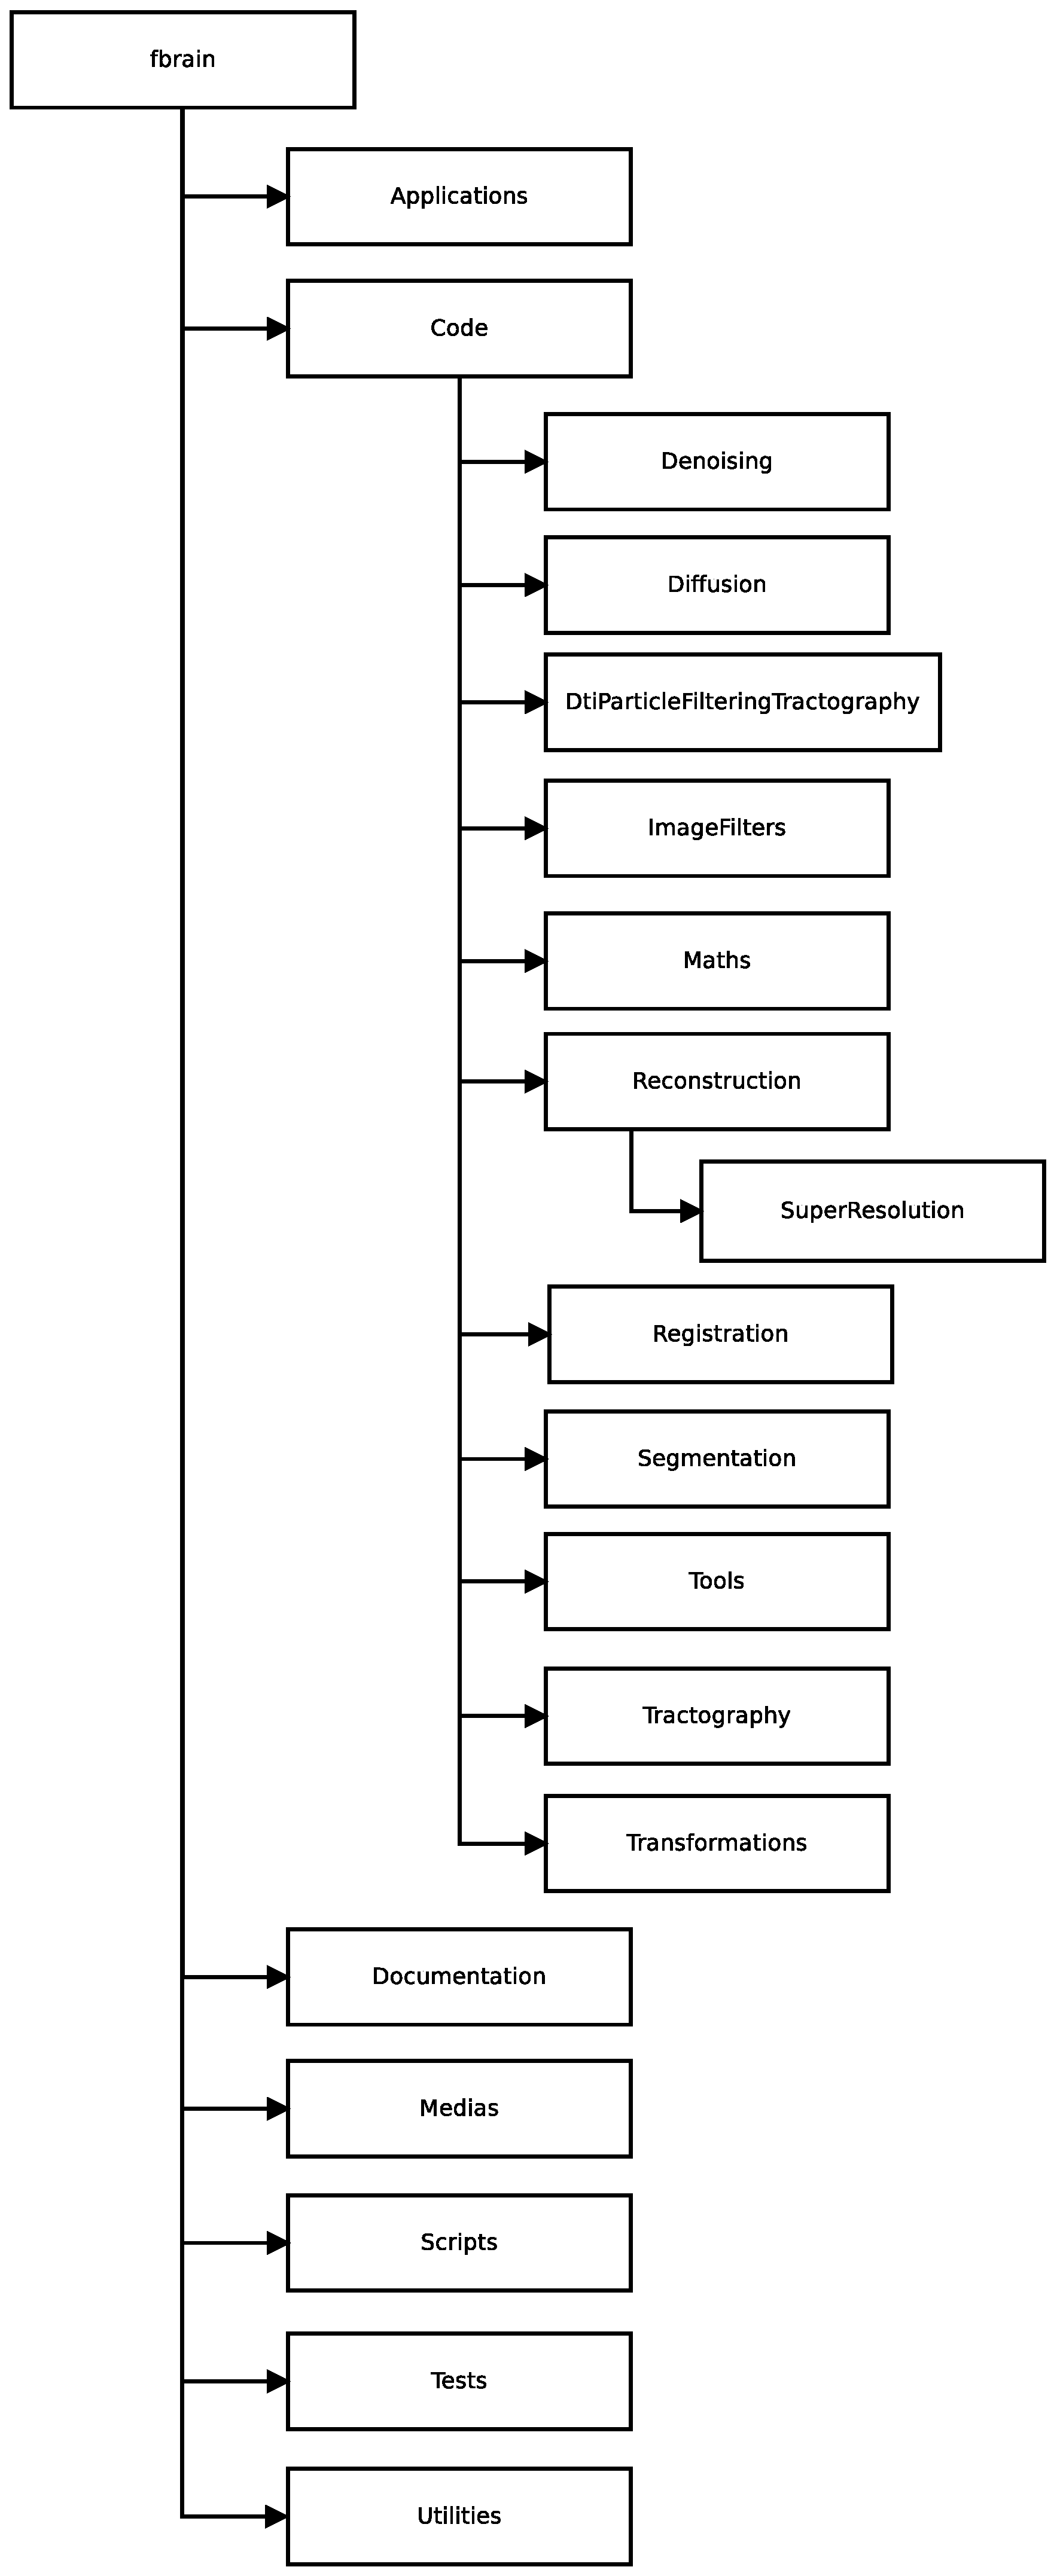
\includegraphics[height=0.5\textwidth]{Btk_tree.eps}
      \caption{Tree of BTK.}
    \end{figure}

    \subsection{Standards}
    Since BTK is written in C++, we use standards, most of time the standards come from ITK library.\\

    \begin{itemize}
    \item Name of Class :\\
      Capital letter at the begining and then CamelCase\footnote{ http://en.wikipedia.org/wiki/CamelCase} :
      \begin{verbatim}
      class MyClass
      class MySuperClass
      \end{verbatim}

    \item Variable member of a Class :\\
      m\_ at the beginin, then a Capital letter and the next in CamelCase :
      \begin{verbatim}
      int m_MyVariable
      \end{verbatim}

    \item Fonction member of a Class :\\
      Capital letter at the begining and then CamelCase :
      \begin{verbatim}
      void MyFonction()
      void MySuperFonction()
      \end{verbatim}

    \item Conditions, loops, instructions... :\\
      Brackets at the line and aligned
      \begin{verbatim}
      for(int i = 0; i < 3; i++)
      {
        //some stuff
      }
      void MySuperFonction()
      {
      
      }
      \end{verbatim}

    \item Constants, enum... :\\
      All letter of the word in capital letter, if composed word separated it by a \_
      \begin{verbatim}
       enum AXES
       {
           AXIAL =0,
           SAGITTAL,
           CORONAL
       } ;

       MY_CONSTANT TRUE = true;
      \end{verbatim}

    \end{itemize}

    Don't forget the C++ standards and be the more logical you can when programming !

    \subsection{Helper classes}
    In BTK we have some helper classes. As their names suggests,those classes are created for helping the programmer for usual fonctions.
    \subsubsection{btkImageHelper}
    \begin{itemize}
    \item File : Code/Tools/btkImageHelper.(h/txx)
    \item Using : Class of static fonctions for create, read, write a image or a vector of images
    \item example :
      \begin{verbatim}
      #include "btkImageHelper.h"
                 
      typedef itk::Image<short, 3> itkImage;
      
      std::string inputFileName = "inputImage.nii.gz";      
      itkImage::Pointer image = btk::ImageHelper<itkImage>::ReadImage(inputFileName);
      
      std::string outputFileName = "outputImage.nii.gz";
      btk::ImageHelper<itkImage>::WriteImage(image, outputFileName);

      \end{verbatim}
    \end{itemize}

    \subsubsection{btkFileHelper}
    \begin{itemize}
    \item File : Code/Tools/btkFileHelper.(h/txx)
    \item Using : Class of static fonctions for check if a file exist or a vector of files
    \item example :
      \begin{verbatim}
      #include "btkFileHelper.h"

      std::string filename("MyName");
      bool fileExist = btk::FileHelper::FileExist(filename);
      \end{verbatim}

    \end{itemize}

    \subsubsection{btkIOTransformHelper}
    \begin{itemize}
    \item File : Code/Tools/btkIOTransformHelper.(h/txx)
    \item Using : Class of static fonctions for reading and writing transforms, this class is currently under developpment !
    \item example :
      \begin{verbatim}
      #include "btkIOTransformHelper.h"

     typedef itk::AffineTransform<double,3> Transform;
     Transform::Pointer transform = Transform::New();
     transform->SetIdentity();

     std string filename("MyName");

     btk::IOTransformHelper<Transform>::WriteTransform(transform,filename);
      
      \end{verbatim}

    \end{itemize}

    \subsubsection{btkMacro}
    \begin{itemize}
    \item File : Code/Tools/btkMacro.h
    \item Using : File with some macro for Set/Get variable into classes
    \item example :
      \begin{verbatim}
      #include "btkMacro.h"

      namespace btk
      {
      class MyClass:
      {
      public:
      // the macro remove the m_ at the begining of the variable
      btkSetMacro(MyVariable,int); 
      btkGetMacro(MyVariable,int);

      private:
      int m_MyVariable;

      };
      }

      \end{verbatim}


    \end{itemize}
  \subsection{Doxygen}
  In order to generate a clear documentation, we using doxygen, so for your classes you should add comments in doxygen spirit.
  Here is a dummy example :
  \begin{verbatim}
#ifndef __MYCLASS_H__
#define __MYCLASS_H__

/*!
 * \file MyClass.h
 * \brief MyClass class
 * \author Luke Skywalker
 * \version 0.1
 */


/*! \namespace btk
 * 
 * namespace to contain all btk composants
 */
namespace btk
{
  /*! \class MyClass
   * \brief class for doing some magical things
   *
   *  Description of the class
   */
  class MyClass
  {
                                               
  public:
    /*!
     *  \brief Constructor
     *
     *  Constructor of the MyClass class
     *
     *  
     */
    MyClass();

    /*!
     *  \brief Destructor
     *
     *  Destructor of the MyClass class
     */
    virtual ~MyClass();

  protected :
  /*!
   *  \brief DoSomething
   *
   *  This method do something
   * \param value : integer value for doing something
   */
  void DoSomething(int value);

  /*!
   *  \brief DoAnotherThing
   *
   *  This method do something
   * \param value : integer value for doing something
   * \return bool : return true if value > 5 else return false
   */
  bool DoAnotherThing(int value);

  private:
  
  int m_MyVariable;/*!< My Variable for doing things*/

  };
};


  \end{verbatim}

     

\subsection{Create a new program}
First of all, you should know that in Btk we have two kind of programs, the first is the \textit{Application} programs which contain the importants programs (for the research project)
and the second is \textit{Utilities} which contain tools and Helpful programs.\\
Creating a new executable program is separated into two steps.
In first you should create a file.cxx which will contained your main
Next you should add your program (and the nessesary includes ) in the corresponding CMake file.\\

\subsubsection{Create a main}
You must create a new file with name of your choice for example btkImageReconstruction.cxx .
If your program take arguments (ie: input/output), you should use TCLAP\footnote{See the documentation http://tclap.sourceforge.net/html/index.html } library.
\subsubsection{Add the programm into CMake}
When your main program is written, you must add it into the CMake file.
Note that there are two CMake files , one for the \textit{Application} and the other for \textit{Utilities}.

Here is a example :
\begin{verbatim}
 ADD_EXECUTABLE(btkTensorStreamlineTractography
        btkTensorStreamlineTractography.cxx
        ${fbrain_SOURCE_DIR}/Code/Tractography/btkCartesianCoordinates.cxx
        ${fbrain_SOURCE_DIR}/Code/Tractography/btkSphericalCoordinates.cxx
        ${fbrain_SOURCE_DIR}/Code/Tractography/btkVector.cxx
        ${fbrain_SOURCE_DIR}/Code/Tractography/btkDirection.cxx
        ${fbrain_SOURCE_DIR}/Code/Tractography/btkPoint.cxx
        ${fbrain_SOURCE_DIR}/Code/DtiParticleFilteringTractography/btkDTFPSignalExtractor.cxx
        ${fbrain_SOURCE_DIR}/Code/DtiParticleFilteringTractography/btkDTFPSignal.cxx
        ${fbrain_SOURCE_DIR}/Code/Tractography/btkSphericalHarmonics.cxx
)

TARGET_LINK_LIBRARIES(btkTensorStreamlineTractography ${ITK_LIBRARIES} vtkHybrid)

INSTALL(TARGETS btkTensorStreamlineTractography
        DESTINATION bin)
\end{verbatim}


..TODO..
